% unit: u35
% sources: sources/076-change-of-basis-image-compression.txt, sources/061-lecture-31-change-of-basis-image-compression.txt, sources/224-mit18-06scf11-ses3-7sum-pdf-download-file.txt, sources/062-problem-solving-change-of-basis.txt, sources/225-mit18-06scf11-ses3-7prob-pdf-download-file.txt, sources/226-mit18-06scf11-ses3-7sol-pdf-download-file.txt
\section{Change of basis; image compression}\label{sec:u35}

Section~\ref{sec:u34} showed that a linear transformation becomes a matrix once a basis is
chosen, and that a better basis gives a better matrix. This unit makes the change from one
basis to another explicit, for vectors (new coordinates) and for transformations (a new,
similar matrix). It starts with the application where the choice of basis is worth billions:
compressing images and video. Recording an image pixel by pixel uses the standard basis, which
is a poor basis for real pictures; switching to a Fourier or wavelet basis lets us keep a few
large coefficients and throw the rest away.

\subsection{Images are vectors, and the standard basis is poor}

A black-and-white image of $512\times512$ pixels records a gray level at every pixel, usually an
integer from $0$ to $255$ (eight bits). The image is therefore a vector $\vb{x}\in\R^n$ with
$n=512^2=262{,}144$ components; a color image needs three times as many. Sending each frame of a
video pixel by pixel would overload any channel.

Giving the value of each pixel is using the standard basis $\vb{e}_1,\dots,\vb{e}_n$: the coefficient of
$\vb{e}_i$ is pixel $i$. This ignores the most important feature of real images, that neighboring
pixels have nearly the same gray level. Before the lecture starts, the camera sees a blank
blackboard: every pixel is (almost) the same. Pixel by pixel that image still costs $n$ numbers.
In a basis that contains the vector of all ones, it costs \emph{one} coefficient. Other useful
basis vectors are the checkerboard $(1,-1,1,-1,\dots)$ and the half-and-half vector
$(1,\dots,1,-1,\dots,-1)$, an image bright on the left and dark on the right. Which basis is best
depends on the signal: the best basis for algebra lectures may not be the best for action films.

\subsection{Transform, threshold, reconstruct}

Lossy compression has three steps, only one of which loses information:
\[
  \underbrace{\vb{x}}_{\text{pixels}}
  \;\xrightarrow{\ \text{change basis (lossless)}\ }\;
  \underbrace{\vb{c}}_{\text{coefficients}}
  \;\xrightarrow{\ \text{threshold (lossy)}\ }\;
  \underbrace{\hat{\vb{c}}}_{\text{many zeros}}
  \;\xrightarrow{\ \text{reconstruct}\ }\;
  \hat{\vb{x}}=\sum_i\hat c_i\vb{w}_i .
\]
The change of basis writes $\vb{x}=c_1\vb{w}_1+\cdots+c_n\vb{w}_n$ in a new basis. \emph{Thresholding} sets
to zero every coefficient below a chosen size, small enough that the eye can hardly see the
difference. A smooth image has a large coefficient on the constant vector (zero frequency) and
very little of the fast-alternating, high-frequency vectors. If $64$ coefficients shrink to $3$,
that is compression by a factor of about $21$.

The JPEG standard (Joint Photographic Experts Group) cuts the $512\times512$ image into $8\times8$
blocks of $64$ pixels and changes basis separately in each block, using cosines: the real parts
of the Fourier vectors of Section~\ref{sec:u30}. Video adds a time dimension. Consecutive frames
are very close, so a good coder predicts each frame from the previous one and encodes only the
small correction. In space or in time, compression exploits the same fact: signals change
smoothly, so neighboring values predict each other.

\subsection{The Haar wavelet basis}

The main competitor to the Fourier basis is a \emph{wavelet} basis. The simplest wavelets, Haar's,
in $\R^8$ are the columns $\vb{w}_1,\dots,\vb{w}_8$ of
\[
  W=\begin{bmatrix*}[r]
  1&1&1&0&1&0&0&0\\
  1&1&1&0&-1&0&0&0\\
  1&1&-1&0&0&1&0&0\\
  1&1&-1&0&0&-1&0&0\\
  1&-1&0&1&0&0&1&0\\
  1&-1&0&1&0&0&-1&0\\
  1&-1&0&-1&0&0&0&1\\
  1&-1&0&-1&0&0&0&-1
  \end{bmatrix*}:
\]
the constant vector, one vector that is $+1$ on the first half and $-1$ on the second, two
that do the same on each half, and four that do it on each quarter
(Figure~\ref{fig:u35-haar}). Every entry is $0$ or $\pm1$, so multiplying by $W$ needs only
additions and subtractions. JPEG2000 uses smoother wavelets built on the same idea.

\begin{figure}[ht]\centering
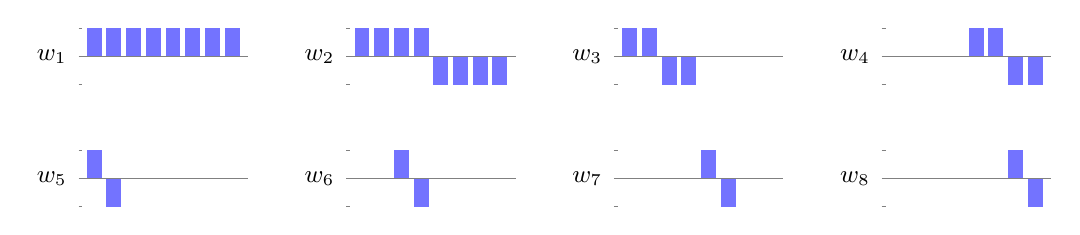
\begin{tikzpicture}[x=0.25cm,y=0.36cm]
  \foreach \vals [count=\i from 0] in
    {{1,1,1,1,1,1,1,1},{1,1,1,1,-1,-1,-1,-1},{1,1,-1,-1,0,0,0,0},{0,0,0,0,1,1,-1,-1},
     {1,-1,0,0,0,0,0,0},{0,0,1,-1,0,0,0,0},{0,0,0,0,1,-1,0,0},{0,0,0,0,0,0,1,-1}} {
    \pgfmathtruncatemacro{\col}{mod(\i,4)}
    \pgfmathtruncatemacro{\row}{int(\i/4)}
    \pgfmathtruncatemacro{\num}{\i+1}
    \begin{scope}[xshift={\col*3.4cm},yshift={-\row*1.55cm}]
      \foreach \h [count=\k from 0] in \vals {
        \fill[blue!55] (\k+0.12,0) rectangle (\k+0.88,\h);
      }
      \draw[gray] (-0.3,0) -- (8.3,0);
      \draw[gray,very thin] (-0.3,1) -- (-0.1,1) (-0.3,-1) -- (-0.1,-1);
      \node[font=\small,anchor=east] at (-0.4,0) {$\vb{w}_{\num}$};
    \end{scope}
  }
\end{tikzpicture}
\caption{The eight Haar wavelets in $\R^8$, drawn as bar charts of their entries ($+1$ up, $-1$
down). Top row: the constant vector and the coarse wavelets on halves and quarters of the
signal. Bottom row: the finest wavelets, each a single $+1,-1$ pair. Their sum
$\vb{w}_5+\vb{w}_6+\vb{w}_7+\vb{w}_8=(1,-1,1,-1,1,-1,1,-1)$ is the fastest-oscillating Fourier vector.}
\label{fig:u35-haar}
\end{figure}

Finding the coefficients of $\vb{x}$ means solving $\vb{x}=W\vb{c}$, so $\vb{c}=W^{-1}\vb{x}$. The Haar vectors make
this easy because they are orthogonal: any two of them overlap where one is constant, and there
the other has as many $+1$'s as $-1$'s, so the dot product is zero.

\begin{proposition}[Coefficients in an orthogonal basis]\label{prop:u35-coeffs}
If $\vb{w}_1,\dots,\vb{w}_n$ is an orthogonal basis of $\R^n$ and $\vb{x}=\sum c_j\vb{w}_j$, then
\[
  c_i=\frac{\vb{w}_i\T\vb{x}}{\vb{w}_i\T\vb{w}_i}.
\]
In matrix form $W\T W=D$ is diagonal and $W^{-1}=D^{-1}W\T$. If the basis is orthonormal, $W^{-1}=W\T$.
\end{proposition}
\begin{proof}
Take the dot product of $\vb{x}=\sum_jc_j\vb{w}_j$ with $\vb{w}_i$. Every term with $j\ne i$ vanishes, leaving
$\vb{w}_i\T\vb{x}=c_i\,\vb{w}_i\T\vb{w}_i$. For the matrix form, the $(i,j)$ entry of $W\T W$ is $\vb{w}_i\T\vb{w}_j$, which is
zero off the diagonal; so $(D^{-1}W\T)W=I$.
\end{proof}

For the Haar basis $\vb{w}_i\T\vb{w}_i$ is $8,8,4,4,2,2,2,2$. Dividing each $\vb{w}_i$ by its length $\sqrt8$,
$\sqrt8$, $2$, $2$, $\sqrt2$, $\sqrt2$, $\sqrt2$, $\sqrt2$ makes $W$ orthogonal, with $W^{-1}=W\T$.

\begin{example}[Compressing eight pixels]\label{ex:u35-compress}
One row of an image has gray levels
\[
  \vb{p}=(100,\,102,\,104,\,106,\,60,\,60,\,62,\,62):
\]
a bright region with a gentle ramp next to a dark region. Using
Proposition~\ref{prop:u35-coeffs}, with $\vb{w}_i\T\vb{w}_i=8,8,4,4,2,2,2,2$:
\begin{align*}
  c_1&=\tfrac18(100+102+104+106+60+60+62+62)=\tfrac{656}{8}=82,\\
  c_2&=\tfrac18\bigl((100+102+104+106)-(60+60+62+62)\bigr)=\tfrac{412-244}{8}=21,\\
  c_3&=\tfrac14\bigl((100+102)-(104+106)\bigr)=-2,\qquad
  c_4=\tfrac14\bigl((60+60)-(62+62)\bigr)=-1,\\
  c_5&=\tfrac12(100-102)=-1,\quad c_6=\tfrac12(104-106)=-1,\quad
  c_7=\tfrac12(60-60)=0,\quad c_8=\tfrac12(62-62)=0 .
\end{align*}
So $\vb{c}=(82,21,-2,-1,-1,-1,0,0)$: the average gray level, the bright/dark contrast, and small
details. \emph{Threshold}: drop every coefficient with $|c_i|\le1$, keeping $\hat{\vb{c}}=(82,21,-2,0,0,0,0,0)$.
\emph{Reconstruct}:
\[
  \hat{\vb{x}}=82\vb{w}_1+21\vb{w}_2-2\vb{w}_3=(101,101,105,105,61,61,61,61).
\]
The error $\vb{p}-\hat{\vb{x}}=(-1,1,-1,1,-1,-1,1,1)$ is at most one gray level out of $255$, invisible,
and three numbers replace eight. A harsher threshold keeping only $c_1$ and $c_2$ gives
$82\vb{w}_1+21\vb{w}_2=(103,103,103,103,61,61,61,61)$, with errors up to $3$
(Figure~\ref{fig:u35-signal}). Had we kept
three \emph{pixels} instead, the other five would be lost entirely.
\end{example}

\begin{figure}[ht]\centering
\begin{tikzpicture}[x=0.9cm,y=0.05cm,>=Stealth]
  \begin{scope}[yshift=-2.5cm]
    \draw[->,gray] (0,50) -- (8.4,50) node[right,font=\small] {pixel};
    \draw[->,gray] (0,50) -- (0,115);
    \foreach \v in {60,80,100} {
      \draw[gray] (-0.08,\v) -- (0.08,\v) node[left=2pt,font=\scriptsize,black] {$\v$};
    }
    \foreach \k in {1,...,8} \node[font=\scriptsize,below] at (\k-0.5,50) {$\k$};
    \draw[thick,dashed,blue] (0,103) -- (4,103) -- (4,61) -- (8,61);
    \draw[very thick,red!75!black] (0,101) -- (2,101) -- (2,105) -- (4,105) -- (4,61) -- (8,61);
    \foreach \x/\v in {0.5/100,1.5/102,2.5/104,3.5/106,4.5/60,5.5/60,6.5/62,7.5/62}
      \fill (\x,\v) circle (2.2pt);
    \node[font=\scriptsize,anchor=west] at (8.6,106) {$\bullet$ pixels $\vb{p}$};
    \node[font=\scriptsize,anchor=west,red!75!black] at (8.6,96) {3 coefficients};
    \node[font=\scriptsize,anchor=west,blue] at (8.6,86) {2 coefficients};
  \end{scope}
\end{tikzpicture}
\caption{The pixel row of Example~\ref{ex:u35-compress} (dots) and its reconstructions from the
largest Haar coefficients. Three coefficients, $82\vb{w}_1+21\vb{w}_2-2\vb{w}_3$ (solid), miss no pixel by
more than one gray level; two coefficients (dashed) keep the bright/dark split but flatten the
ramp.}
\label{fig:u35-signal}
\end{figure}

What makes a basis good for compression? Two properties, and the competition between bases
is about both:
\begin{enumerate}
  \item \emph{Fast}: multiplying by $W$ and by $W^{-1}$ must be cheap. The Fourier basis has the FFT
        (Section~\ref{sec:u30}); wavelets have a fast wavelet transform; orthonormal bases have
        $W^{-1}=W\T$. The fastest choice of all is to change nothing, the standard basis, which fails
        the second test.
  \item \emph{Good compression}: a few basis vectors should come close to the signal, so that most
        coefficients are small and can be set to zero.
\end{enumerate}
The ideal basis would be the eigenvectors of a matrix built from the image itself, but finding
them costs far more than the savings; Fourier and wavelet bases are cheap and close.

\subsection{Change of basis for vectors and for transformations}

\emph{Vectors.} Let the columns of $W$ be new basis vectors $\vb{w}_1,\dots,\vb{w}_n$ of $\R^n$. A vector with
standard coordinates $\vb{x}$ has new coordinates $\vb{c}$ related by
\[
  \vb{x}=W\vb{c},\qquad \vb{c}=W^{-1}\vb{x}.
\]

\emph{Transformations.} Now let $T\colon V\to V$ be linear and use the same basis for inputs and
outputs. In an old basis $\vb{v}_1,\dots,\vb{v}_n$ it has a matrix $A$, in a new basis $\vb{w}_1,\dots,\vb{w}_n$ a
matrix $B$. The same transformation should give closely related matrices, and it does.

\begin{theorem}[Changing basis gives a similar matrix]\label{thm:u35-similar}
Let $M$ be the matrix whose column $j$ holds the old coordinates of the new basis vector $\vb{w}_j$.
Then for every vector, $(\text{old coordinates})=M\,(\text{new coordinates})$, and
\[
  B=M^{-1}AM .
\]
\end{theorem}
\begin{proof}
If $\vb{x}=\sum_jd_j\vb{w}_j$, substituting $\vb{w}_j=\sum_iM_{ij}\vb{v}_i$ gives
$\vb{x}=\sum_i\bigl(\sum_jM_{ij}d_j\bigr)\vb{v}_i$, so the old coordinates are $M\vb{d}$. Since $M$ converts
coordinates of a basis into coordinates of a basis, it is invertible. Now follow
Figure~\ref{fig:u35-diagram}: start with new coordinates $\vb{d}$ of $\vb{x}$; $M\vb{d}$ are its old coordinates;
$AM\vb{d}$ are the old coordinates of $T(\vb{x})$ (Section~\ref{sec:u34}); $M^{-1}AM\vb{d}$ are the new coordinates
of $T(\vb{x})$. A matrix that turns the new coordinates of every $\vb{x}$ into the new coordinates of
$T(\vb{x})$ is the matrix $B$ (apply it to $\vb{d}=\vb{e}_j$ to recover column $j$). So $B=M^{-1}AM$.
\end{proof}

\begin{figure}[ht]\centering
\begin{tikzpicture}[>=Stealth,font=\small]
  \node (nx) at (0,1.6) {new coordinates of $\vb{x}$};
  \node (ox) at (6,1.6) {old coordinates of $\vb{x}$};
  \node (nT) at (0,0) {new coordinates of $T(\vb{x})$};
  \node (oT) at (6,0) {old coordinates of $T(\vb{x})$};
  \draw[->,thick] (nx) -- node[above] {$M$} (ox);
  \draw[->,thick] (ox) -- node[right] {$A$} (oT);
  \draw[->,thick] (oT) -- node[below] {$M^{-1}$} (nT);
  \draw[->,thick,red!75!black] (nx) -- node[left] {$B=M^{-1}AM$} (nT);
\end{tikzpicture}
\caption{Two routes from the new coordinates of $\vb{x}$ to the new coordinates of $T(\vb{x})$: directly by
$B$, or by translating to the old basis ($M$), applying $A$, and translating back ($M^{-1}$).
Because both routes agree, $B=M^{-1}AM$: the two matrices of one transformation are similar.}
\label{fig:u35-diagram}
\end{figure}

This is where similar matrices (Section~\ref{sec:u32}) really come from: they are the matrices of
one transformation in different bases, which is why they share eigenvalues, trace and
determinant, all of which belong to $T$ itself. The best basis is again the eigenvector basis:
if $T(\vb{v}_i)=\lambda_i\vb{v}_i$, then column $i$ of the matrix is $\lambda_i\vb{e}_i$ and the matrix is $\Lambda$.

\begin{example}[Diagonalizing a projection by a change of basis]\label{ex:u35-projection}
In the standard basis the projection onto the $45^\circ$ line has matrix
$A=\left[\begin{smallmatrix}1/2&1/2\\1/2&1/2\end{smallmatrix}\right]$ (Section~\ref{sec:u34}). Take the new basis
$\vb{w}_1=(1,1)$ on the line and $\vb{w}_2=(-1,1)$ across it, so $M=\left[\begin{smallmatrix}1&-1\\1&1\end{smallmatrix}\right]$ and
$M^{-1}=\tfrac12\left[\begin{smallmatrix}1&1\\-1&1\end{smallmatrix}\right]$. Then
\[
  AM=\begin{bmatrix}1&0\\1&0\end{bmatrix},\qquad
  B=M^{-1}AM=\frac12\begin{bmatrix}1&1\\-1&1\end{bmatrix}\begin{bmatrix}1&0\\1&0\end{bmatrix}=\begin{bmatrix}1&0\\0&0\end{bmatrix}=\Lambda .
\]
\end{example}

\begin{example}[A basis known only by its values]\label{ex:u35-lagrange}
In the space of polynomials of degree at most $2$, compare the basis $1,x,x^2$ with a basis
$\vb{w}_1,\vb{w}_2,\vb{w}_3$ known only through its values at $x=-1,0,1$:
\[
  \begin{array}{c|ccc}
    & x=-1 & x=0 & x=1\\\hline
    \vb{w}_1 & 1&0&0\\ \vb{w}_2&0&1&0\\ \vb{w}_3&0&0&1
  \end{array}
\]
\emph{New coordinates are values.} If $p=\alpha\vb{w}_1+\beta\vb{w}_2+\gamma\vb{w}_3$, evaluating at $-1,0,1$ gives
$p(-1)=\alpha$, $p(0)=\beta$, $p(1)=\gamma$. So $y=5-x$, with values $6,5,4$, is $y=6\vb{w}_1+5\vb{w}_2+4\vb{w}_3$.

\emph{Change of basis matrices.} The new coordinates of $1$, $x$, $x^2$ are their values:
$(1,1,1)$, $(-1,0,1)$, $(1,0,1)$. These are the columns of $M^{-1}$ (old $\to$ new), and inverting
gives $M$ (new $\to$ old), whose columns are the $\vb{w}$'s written in $1,x,x^2$:
\[
  M^{-1}=\begin{bmatrix*}[r]1&-1&1\\1&0&0\\1&1&1\end{bmatrix*},\qquad
  M=\begin{bmatrix*}[r]0&1&0\\-\tfrac12&0&\tfrac12\\\tfrac12&-1&\tfrac12\end{bmatrix*},
\]
that is $\vb{w}_1=\tfrac12(x^2-x)$, $\vb{w}_2=1-x^2$, $\vb{w}_3=\tfrac12(x^2+x)$. (Check $\vb{w}_1$: values
$\tfrac12(1+1)=1$, $0$, $\tfrac12(1-1)=0$.)

\emph{The derivative in both bases.} With $1,x,x^2$ for inputs and outputs, $T=\frac{d}{dx}$ has
$A=\left[\begin{smallmatrix}0&1&0\\0&0&2\\0&0&0\end{smallmatrix}\right]$. In the $\vb{w}$ basis,
\[
  B=M^{-1}AM=\begin{bmatrix*}[r]-\tfrac32&2&-\tfrac12\\-\tfrac12&0&\tfrac12\\\tfrac12&-2&\tfrac32\end{bmatrix*}.
\]
Column~1 should be the values of $\vb{w}_1'=x-\tfrac12$ at $-1,0,1$: $(-\tfrac32,-\tfrac12,\tfrac12)$. It is.
And $B(6,5,4)=(-9+10-2,\ -3+0+2,\ 3-10+6)=(-1,-1,-1)$, the values of $y'=-1$. Both $A$ and $B$ have
trace $0$ and only the eigenvalue $0$, as similar matrices must.
\end{example}

\begin{trap}
Keep the direction of $M$ straight. Its columns are the \emph{new} basis vectors written in the
\emph{old} coordinates, so $M$ converts new coordinates to old ($\vb{x}=W\vb{c}$ in $\R^n$), and the new matrix
is $M^{-1}AM$, not $MAM^{-1}$. A quick test: apply your formula for $B$ to $\vb{e}_1$ and check that it
gives the new coordinates of $T(\vb{w}_1)$.
\end{trap}

\subsection{Exercises}

\begin{exercise}[An orthonormal Haar basis]\label{exr:u35-haar}
Verify that the eight Haar vectors are orthogonal and rescale them to an orthonormal basis.
\end{exercise}
\begin{solution}
$\vb{w}_2,\dots,\vb{w}_8$ each have equally many $+1$'s and $-1$'s, so they are orthogonal to the constant
$\vb{w}_1$. Each of $\vb{w}_3,\dots,\vb{w}_8$ lives on one half of the signal, where $\vb{w}_2$ is constant, and has
equally many $\pm1$ there, so it is orthogonal to $\vb{w}_2$. The same argument on quarters handles
$\vb{w}_3,\vb{w}_4$ against $\vb{w}_5,\dots,\vb{w}_8$, and vectors with disjoint supports (such as $\vb{w}_3$ and $\vb{w}_4$,
or $\vb{w}_5$ and $\vb{w}_6$) have dot product $0$. The lengths are $\sqrt8,\sqrt8,2,2,\sqrt2,\sqrt2,\sqrt2,\sqrt2$,
so the orthonormal basis is $\vb{w}_1/\sqrt8$, $\vb{w}_2/\sqrt8$, $\vb{w}_3/2$, $\vb{w}_4/2$, $\vb{w}_5/\sqrt2,\dots,\vb{w}_8/\sqrt2$:
entries $\pm1/\sqrt8$, $\pm\tfrac12$ and $\pm1/\sqrt2$.
\end{solution}

\begin{exercise}[Lossless compression]\label{exr:u35-lossless}
Find the Haar coefficients of $\vb{p}=(4,4,4,4,2,2,0,0)$. How many numbers are needed to store $\vb{p}$
exactly?
\end{exercise}
\begin{solution}
$c_1=\tfrac18(16+4)=2.5$, $c_2=\tfrac18(16-4)=1.5$, $c_3=\tfrac14(8-8)=0$, $c_4=\tfrac14(4-0)=1$, and
$c_5=c_6=c_7=c_8=0$ since each neighbouring pair is equal. So $\vb{p}=2.5\vb{w}_1+1.5\vb{w}_2+\vb{w}_4$, three numbers
with no loss at all. Check the fifth entry: $2.5-1.5+1=2$.
\end{solution}

\begin{exercise}[Bases for \texorpdfstring{$2\times2$}{2 by 2} matrices]\label{exr:u35-matrices}
The $2\times2$ real matrices form a four-dimensional vector space. Give two different bases. Which
is better for describing diagonal matrices? Triangular ones? Symmetric ones?
\end{exercise}
\begin{solution}
The standard basis is $\left[\begin{smallmatrix}1&0\\0&0\end{smallmatrix}\right]$,
$\left[\begin{smallmatrix}0&1\\0&0\end{smallmatrix}\right]$, $\left[\begin{smallmatrix}0&0\\1&0\end{smallmatrix}\right]$,
$\left[\begin{smallmatrix}0&0\\0&1\end{smallmatrix}\right]$. Another is
$\left[\begin{smallmatrix}1&0\\0&1\end{smallmatrix}\right]$, $\left[\begin{smallmatrix}0&1\\1&0\end{smallmatrix}\right]$,
$\left[\begin{smallmatrix}1&0\\0&-1\end{smallmatrix}\right]$, $\left[\begin{smallmatrix}0&1\\-1&0\end{smallmatrix}\right]$; viewed as
vectors in $\R^4$ these are orthogonal, hence independent. The standard basis is best for
diagonal matrices (two basis elements suffice) and for triangular ones (three). The second basis
is also good for diagonal matrices, e.g.\ $\left[\begin{smallmatrix}4&0\\0&2\end{smallmatrix}\right]
=3\left[\begin{smallmatrix}1&0\\0&1\end{smallmatrix}\right]+1\left[\begin{smallmatrix}1&0\\0&-1\end{smallmatrix}\right]$, and it is the
best for symmetric matrices: they are exactly the combinations with coefficient $0$ on the
antisymmetric $\left[\begin{smallmatrix}0&1\\-1&0\end{smallmatrix}\right]$.
\end{solution}

\begin{exercise}[A rotation in a reflected basis]\label{exr:u35-rotation}
The rotation by $90^\circ$ has standard matrix $R=\left[\begin{smallmatrix}0&-1\\1&0\end{smallmatrix}\right]$. Find its
matrix in the basis $\vb{w}_1=(1,1)$, $\vb{w}_2=(1,-1)$, and explain the answer.
\end{exercise}
\begin{solution}
$M=\left[\begin{smallmatrix}1&1\\1&-1\end{smallmatrix}\right]$, $M^{-1}=\tfrac12\left[\begin{smallmatrix}1&1\\1&-1\end{smallmatrix}\right]$,
$RM=\left[\begin{smallmatrix}-1&1\\1&1\end{smallmatrix}\right]$, and
$B=M^{-1}RM=\tfrac12\left[\begin{smallmatrix}0&2\\-2&0\end{smallmatrix}\right]=\left[\begin{smallmatrix}0&1\\-1&0\end{smallmatrix}\right]$.
Directly: $R\vb{w}_1=(-1,1)=-\vb{w}_2$ and $R\vb{w}_2=(1,1)=\vb{w}_1$, which are the columns $(0,-1)$ and $(1,0)$. The
new matrix looks like rotation by $-90^\circ$ because the basis $\vb{w}_1,\vb{w}_2$ has the opposite
orientation ($\det M=-2<0$). Trace $0$ and determinant $1$ are unchanged, as they must be.
\end{solution}
